\section{Verifikation von Implementierungen}

\subsection{Symbolische Ausführung in Verifast}

Die Verifizierung von Implementierungs-Code findet in Verifast über eine symbolische Ausführung statt.
Dabei wird mit den Vorbedingungen des Methodenvertrags gestartet und versucht daraus die
Nachbedingungen abzuleiten.

Der aktuelle Zustand der Ausführung wird dabei durch zwei verschiedene Strukturen charakterisiert: 
Den Heap, der alle Elemente (engl. heap chunks) des Speichers beinhaltet sowie eine Liste
der geschlussfolgerten Annahmen (engl. assumptions). Bei der Ausführung der Vorbedingungen werden
diese Aussagen nun untersucht und entweder zum Heap hinzugefügt oder zu den Annahmen.

Beim Verstehen dieser Schritte ist die Verifast-Oberfläche sehr hilfreich, da sie den aktuellen
Zustand für einen beliebigen Haltepunkt anzeigen kann. Die folgende Situation zeigt die Ausführung
einer \lstinline{mismatch}-Implementierung bis zum gesetzten Haltepunkt (gelb hervorgehoben).

\begin{center}
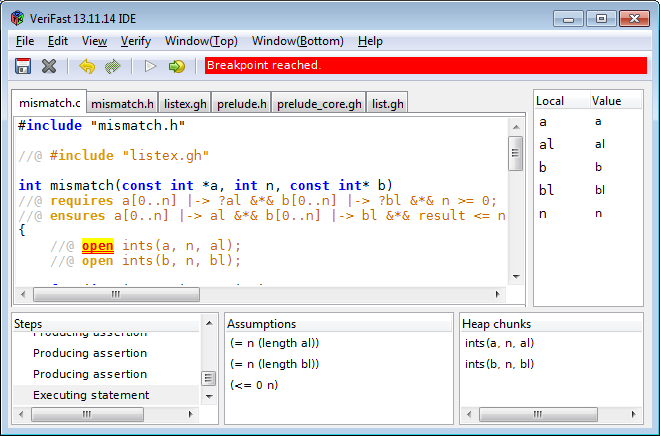
\includegraphics[width=1.0\textwidth]{images/verifast-state-after-precondition.png}
\end{center}

Gut zu erkennen ist, dass logische Ausdrücke wie \(n >= 0\) in die Liste der Annahmen 
(im Bild als \glqq Assumptions\grqq betitelt) aufgenommen wurden. Die \lstinline{ints}-Prädikate hingegen
wurden zum Heap hinzugefügt. Diesen Prozess nennt Verifast \glqq Producing assertion\grqq, wobei sich das Verb
\glqq Producing\grqq auf das Hinzufügen von Elementen zum aktuellen Zustand der symbolischen Ausführung
bezieht.

Das Gegenteil - \glqq Consuming assertion\grqq - findet z.B. beim Verifizieren der Nachbedingungen statt.
Verifast versucht dann alle erforderlichen Aussagen in der Liste der Annahmen bzw. im Heap zu finden
und diese, wenn sie denn passen, zu entfernen. Zusätzlich dazu wird am Ende einer Funktion - beim 
\glqq Leak check\grqq - auch überprüft, dass der Heap (der aktuellen Funktion) leer ist. Ist das nicht 
der Fall so wurde der entsprechende Speicher nicht korrekt bereinigt oder zumindest war Verifast nicht 
in der Lage das Gegenteil zu beweisen.

In dem Fall von mismatch würde Verifast die Heap chunks \lstinline{ints(a, n, al)} sowie
\lstinline{ints(b, n, bl)} beim Konsumieren der Nachbedingung auf dem Heap finden, entfernen und
somit erfolgreich verifizieren können, dass der Speicher so wie vor dem Aufruf vorhanden ist.



prädikate sind typen auf dem symbol heap

ghost commands zum öffnen und schließen

\subsection{Rekursive equal-Implementierung}

\todo{in acsl werden vor- und nachbedingung separat ausgewertet, auf grund der rückwärtsverifikation}


präzise prädikate sparent schreibaufwand

code zeigen

rekursion meist einfacher zu beweisen

\subsection{ACSL-Implementierung im Vergleich}

rekursive implementierung mit acsl zeigen

toolunterstützung frama-c zeigen und erklären

\subsection{Schleifeninvarianten}

schleifeninvarianten in acsl

alle angefassten variablen müssen per assigns erlaubt werden

dann in verifast zeigen

ähnlich, alles muss in invariante defniiert sein, was man benutzen will

\subsection{Lemmata und Axiome}

fixpoint nochmal zeigen (take)

erwähnen dass verifast terminierung von fixpount und lemmas prüft

\lstinline{take_one_plus} lemma zeigen

ggf. screenshot hier erst zeigen

erklären wieso es notwendig ist

\subsection{Speicherprobleme aufdecken}

malloc/free - chunks

zeigen an hand von main-funktion (unit-test)

verifast hilft klar zu dokumentieren wer für speicher verantwortlich ist (rufer oder gerufener)

\subsection{Überläufe erkennen}

overflow checken
